\chapter{Религия, Рим и Цезарь}

Я не раз отмечал что римляне были очень религиозными людьми. Практически лишенные средневекового ханжества и этого угрюмого христианского "бубубу", но относящиеся к религиозным вопросам и ритуалам крайне серьезно. Максимально. Настолько, что не вовремя трахнувший жену Цезаря Клодий вызвал жесточайший политический кризис и на месяц фактически остановил работу Республики. А проиллюстрировать этот тезис нам поможет сам Гай Юлий, а точнее сцена его убийства.

\begin{figure}[h!tb] 
	\centering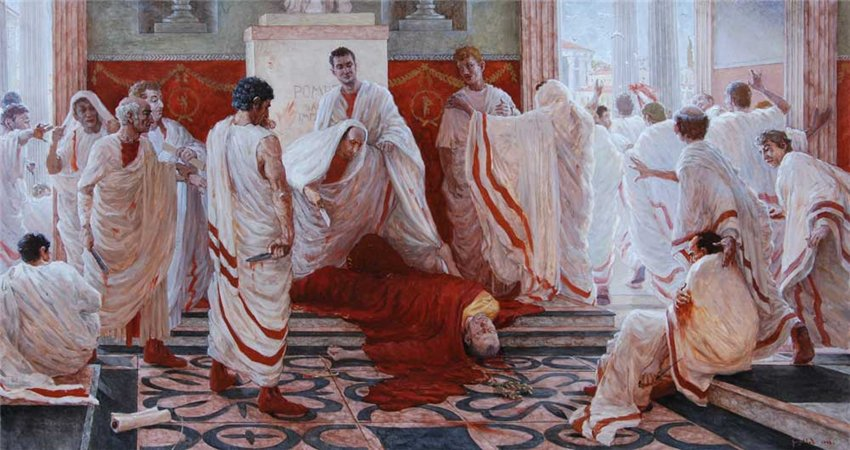
\includegraphics[scale=0.6]{ReligionRomeCaesar/15957456631798748.png}
	%	\label{fig:scipion} % Unique label used for referencing the figure in-text\end{document}
	%	%\addcontentsline{toc}{figure}{Figure \ref{fig:placeholder}} % Uncomment to add the figure to the table of contents%----------------------------------------------------------------------------------------
	\caption{На пикчах ниже всякие вариации на тему "сенаторы убивают Салата".}%	CHAPTER 2
\end{figure}
Не секрет что к "свержению тирана" господа заговорщики подошли очень серьезно. Это не просто "придти да зарезать старикана ножиками", нет. Это — ритуал, почти жертвоприношение. Для этого дела собрали представителей почти всех старых аристократических фамилий, стоящих у основания Республики. Тоесть они, коллективно, могли проследить родословную чуть ли не к любому из первой плеяды сенаторов, которые "изгнали царей, спасли Рим и создали Республику". И, как вишенка на торте - Марк Юний Брут, прямой потомок Луция Юния Брута, который лично убил последнего царя (и в честь которого, по одной из версий, назван месяц июнь). Каждый из заговорщиков должен нанести ровно по одному удару. И больше никто не должен был пострадать (что, кстати, очень сильно им повредило, так как начни они убивать цезарианских вождей сразу, то шансов было куда больше. В первую очередь резать надо было Лепида и Антония, канешно). В общем, это было не убийство а ритуальное мероприятие, отыгрывался классический сюжет из преданий, только заговорщики тут живые, диктатор тоже живой, и убийство настоящее. 

\begin{figure}[h!tb] 
	\centering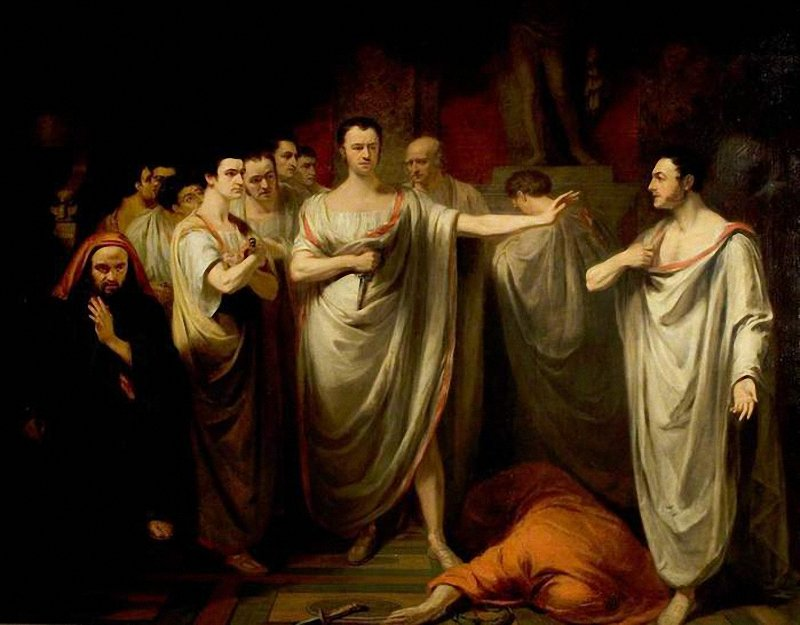
\includegraphics[scale=0.5]{ReligionRomeCaesar/159574567419687932.png}
	%	\label{fig:scipion} % Unique label used for referencing the figure in-text\end{document}
	%	%\addcontentsline{toc}{figure}{Figure \ref{fig:placeholder}} % Uncomment to add the figure to the table of contents%----------------------------------------------------------------------------------------
	%	\caption{На пикчах ниже всякие вариации на тему "сенаторы убивают Салата".}%	CHAPTER 2
\end{figure}

Многие, особенно те кто этой замечательной римской любви к ритуалам не понимает, списывают поведение убийц на голый популизм и немножко идиотизм. Но я обращаю внимание на то, что для черни это было вообще похеру, эти как раз были людьми "низкой культуры дискуссии". И, прямо скажем, совершенно не оценили такую ритуальность, немедленно попытавшись разорвать виновников на куски. Не дало это особых преимуществ и потом, так как по политическим соображениям (Антоний встал во главе городского плебса и контролировал Народное Собрание, а Лепид стоял за Рубиконом с армией. Оба ярые цезарианцы и с обоими пришлось договариваться) пришлось как-то мямлить народу про то что убийство не убийство а диктатор не диктатор, и так далее. Я об этом писал в тексте про Октавиана более подробно. В общем, еслиб убивали Цезаря более прозаично и менее ритуально, то пользы былоб сильно больше. Но так уж сложилось, что всё надо было обставить по феншую, даже если это сулит самые нехорошие последствия. 


\begin{figure}[h!tb] 
	\centering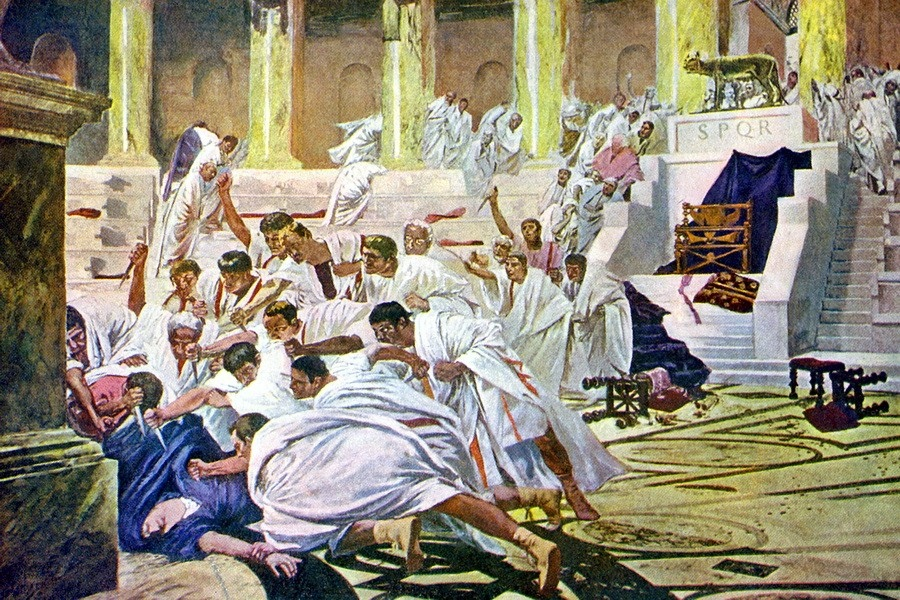
\includegraphics[scale=0.4]{ReligionRomeCaesar/159574567611657516.png}
	%	\label{fig:scipion} % Unique label used for referencing the figure in-text\end{document}
	%	%\addcontentsline{toc}{figure}{Figure \ref{fig:placeholder}} % Uncomment to add the figure to the table of contents%----------------------------------------------------------------------------------------
	%	\caption{На пикчах ниже всякие вариации на тему "сенаторы убивают Салата".}%	CHAPTER 2
\end{figure}

А теперь внимание, к чему была эта подводка? Дело в том, что, ЦЕЗАРЬ ТОЖЕ ВОСПРИНЯЛ СВОЁ УБИЙСТВО КАК РИТУАЛЬНОЕ ДЕЙСТВО. Когда он понял что его сейчас начнут резать, то не попытался убежать или отмахаться. Не тянул время, не пытался никого уговаривать, а, так сказать, "стоически принял свою судьбу". Да и до заговора фатализм так и прет. Настолько, что есть версия о том, что весь заговор был им инсценирован самостоятельно чтобы заговорщики после того как он отъедет в Парфию - начали действовать и дали повод устроить в Риме резню (для чего и нужен был Лепид с армией в Цизальпийской Галлии, например). В общем, эта версия звучит достаточно логично именно потому, что он просто игнорировал кучу как косвенных так и прямых свидетельств готовящегося, причем как религиозных предзнаменований, так и вполне обыденных доносов. Но даже если предположить что всё это - неудачная многоходовочка Цезаря, вышедшая из под контроля, то действия во время самого убийства укладываются только в "ритуальную" версию.

\begin{figure}[h!tb] 
	\centering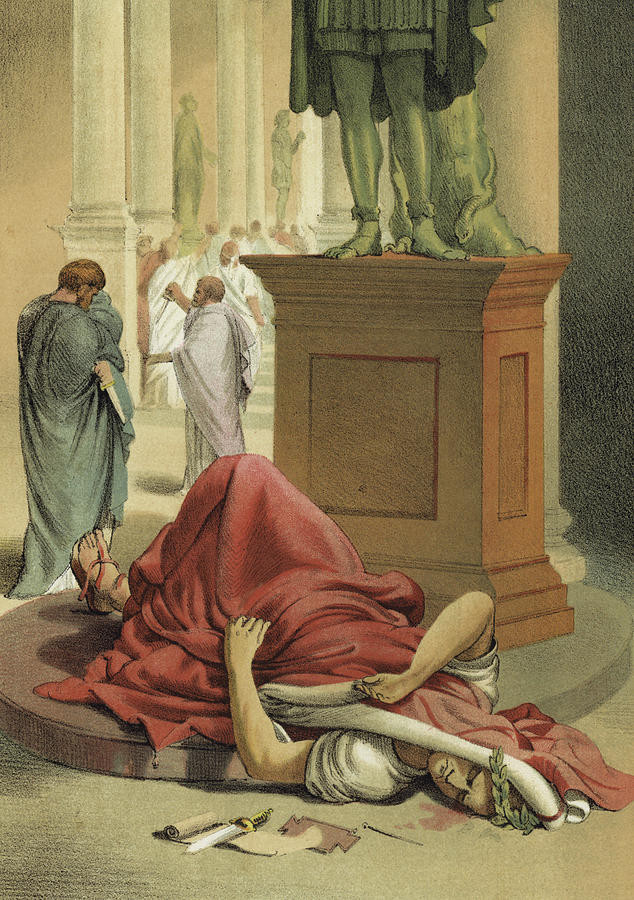
\includegraphics[scale=0.4]{ReligionRomeCaesar/1595745697116880936.jpg}
	%	\label{fig:scipion} % Unique label used for referencing the figure in-text\end{document}
	%	%\addcontentsline{toc}{figure}{Figure \ref{fig:placeholder}} % Uncomment to add the figure to the table of contents%----------------------------------------------------------------------------------------
	%	\caption{На пикчах ниже всякие вариации на тему "сенаторы убивают Салата".}%	CHAPTER 2
\end{figure}

Судите сами.
Вот так Салюстрий описывает события после первого удара ножом:
\textit{"Когда же он увидел, что со всех сторон на него направлены обнаженные кинжалы, он накинул на голову тогу и левой рукой распустил ее складки ниже колен (!), чтобы пристойнее упасть укрытым до пят; и так он был поражен двадцатью тремя ударами, только при первом испустив не крик даже, а стон. }


\begin{figure}[h!tb] 
	\centering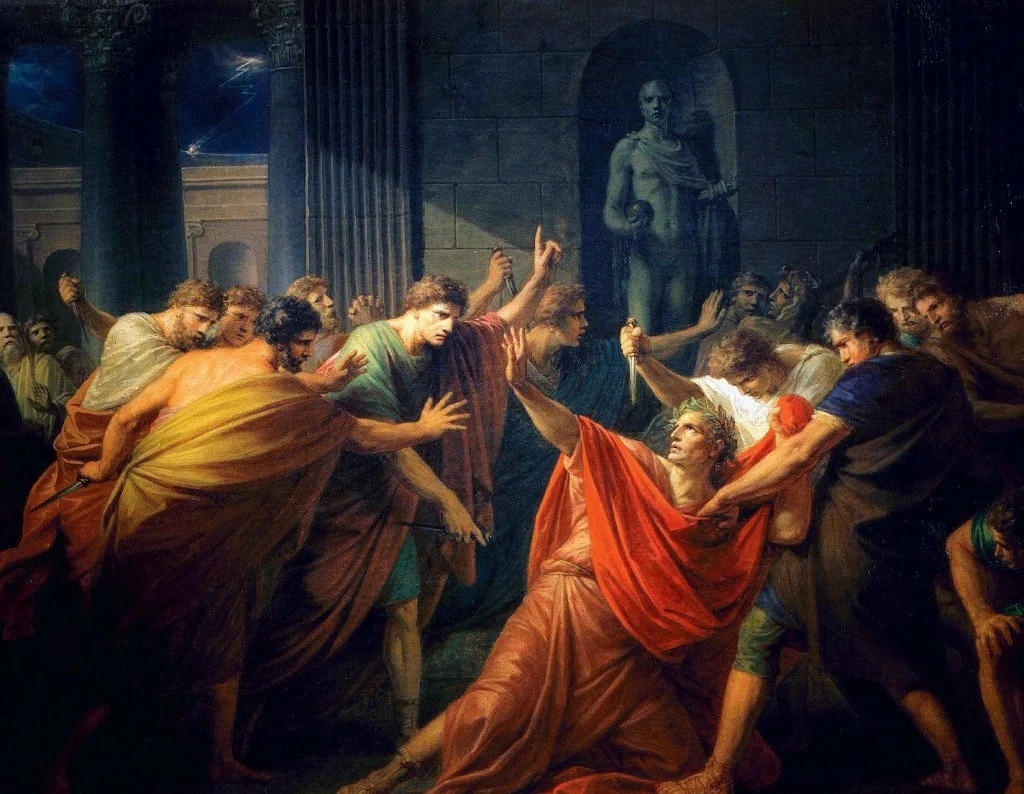
\includegraphics[scale=0.4]{ReligionRomeCaesar/1595745702141158794.png}
	%	\label{fig:scipion} % Unique label used for referencing the figure in-text\end{document}
	%	%\addcontentsline{toc}{figure}{Figure \ref{fig:placeholder}} % Uncomment to add the figure to the table of contents%----------------------------------------------------------------------------------------
	%	\caption{На пикчах ниже всякие вариации на тему "сенаторы убивают Салата".}%	CHAPTER 2
\end{figure}




Вот Аппиан, тут немножко другая инфа, и Цезарь перестает сопротивляться после того как увидел Брута:
\textit{"Цезарь, как дикий зверь, поворачивался от одного к другому. Но после удара Брута… он закрылся со всех сторон плащом (!) и упал, сохраняя пристойный вид, перед статуей Помпея. Заговорщики превзошли всякую меру в отношении к павшему и нанесли ему до 23 ран. Многие в суматохе ранили мечами друг друга"}

\begin{figure}[h!tb] 
	\centering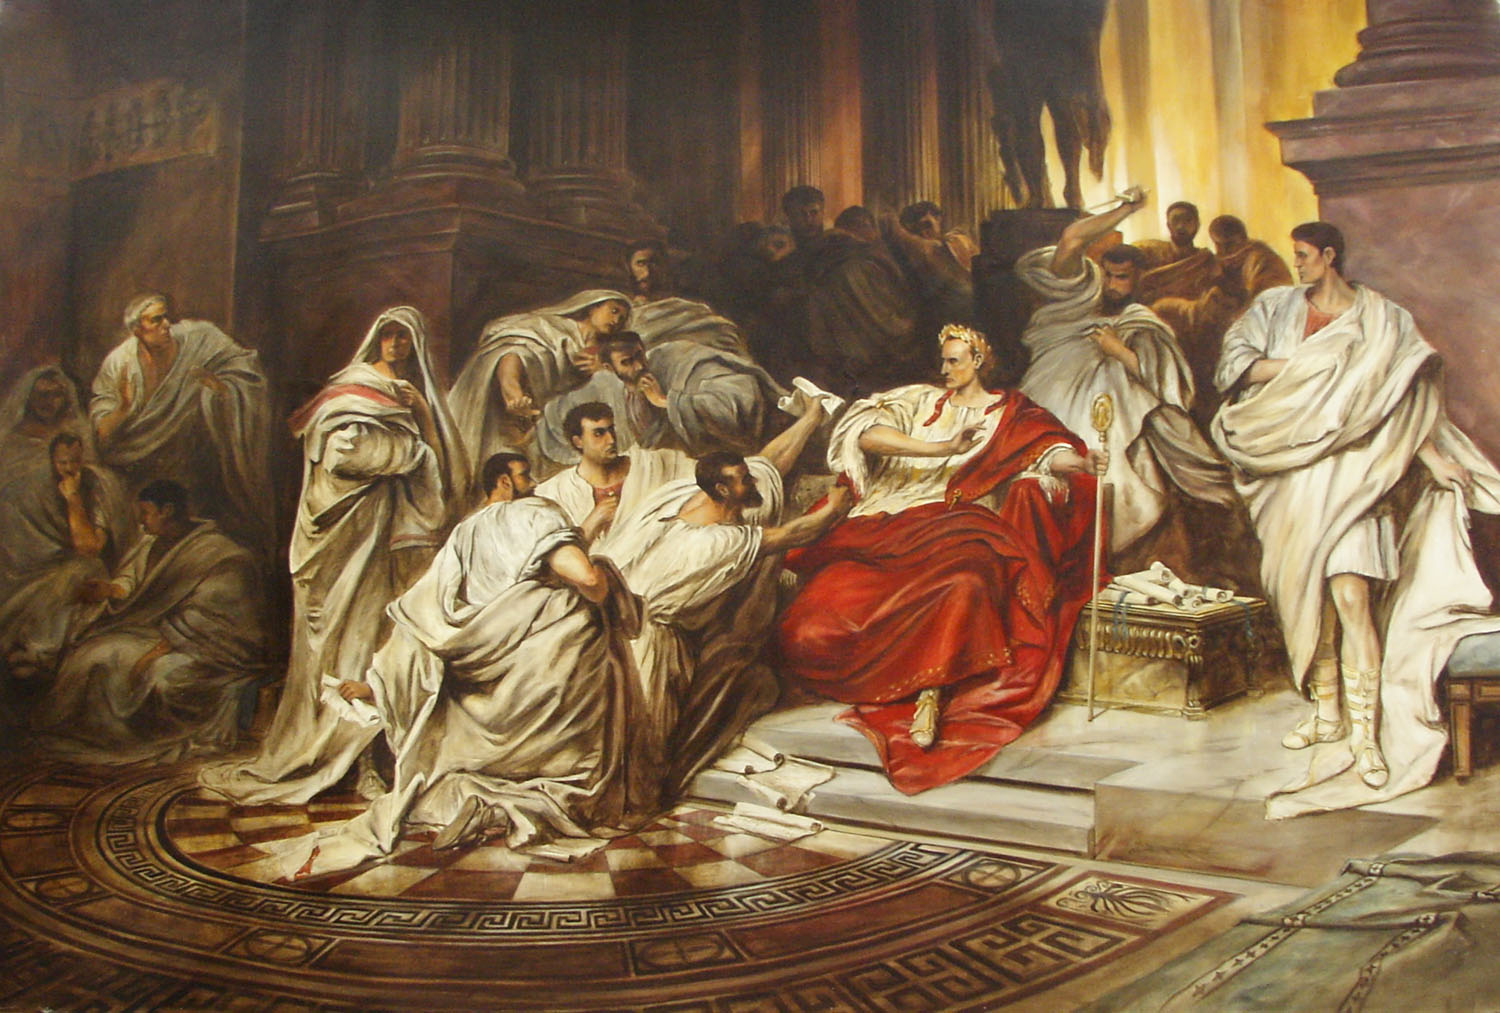
\includegraphics[scale=0.3]{ReligionRomeCaesar/1595745705118471335.png}
	%	\label{fig:scipion} % Unique label used for referencing the figure in-text\end{document}
	%	%\addcontentsline{toc}{figure}{Figure \ref{fig:placeholder}} % Uncomment to add the figure to the table of contents%----------------------------------------------------------------------------------------
	%	\caption{На пикчах ниже всякие вариации на тему "сенаторы убивают Салата".}%	CHAPTER 2
\end{figure}



А вот Плутарх, тут тоже Брут сработал как спусковой механизм:

\textit{"Некоторые писатели рассказывают, что, отбиваясь от заговорщиков, Цезарь метался и кричал, но, увидев Брута с обнаженным мечом, накинул на голову тогу и подставил себя под удары (!). Либо сами убийцы оттолкнули тело Цезаря к цоколю, на котором стояла статуя Помпея, либо оно там оказалось случайно. Цоколь был сильно забрызган кровью. Можно было подумать, что сам Помпей явился для отмщенья своему противнику, распростертому у его ног, покрытому ранами и еще содрогавшемуся."} 

Во всех трех цитатах я отметил интересующее меня восклицательными знаками. Как только Цезарь понимает что происходит не какая-то херня, а самое настоящее ритуальное убийство с ним в главные роли, он эту роль немедленно принимает и ведет себя соответственно, тоесть с достоинством и без суеты. Как настоящий римский патриций былых эпох. Вот такая у людей была стальная воля, и отношение к жизни и смерти. Причем это не что-то удивительное, а общее для тех времен явление, и наверное поэтому поведение Цезаря не казалось чем-то из ряда вон выходящим.


\begin{figure}[h!tb] 
	\centering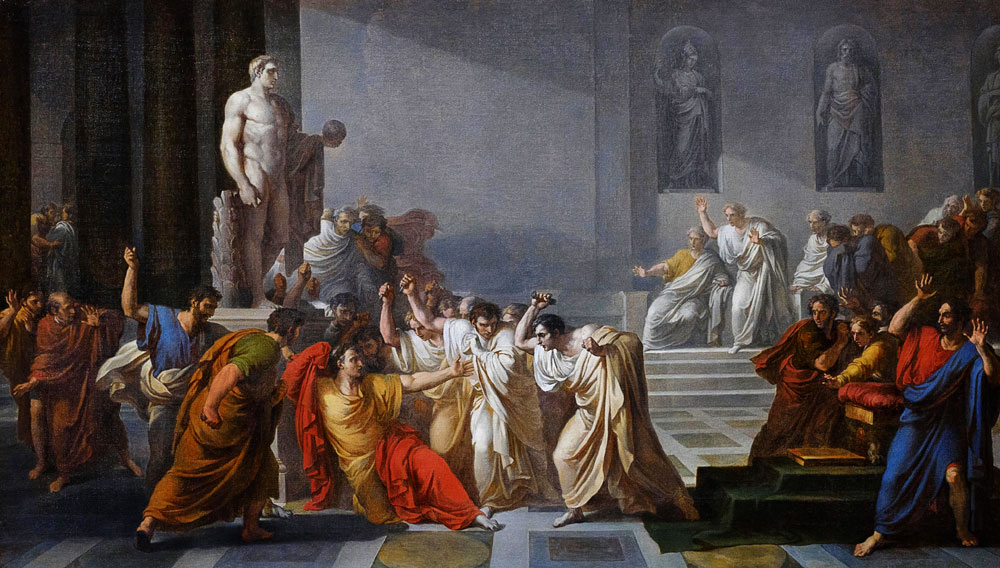
\includegraphics[scale=0.4]{ReligionRomeCaesar/1595745699111517977.png}
	%	\label{fig:scipion} % Unique label used for referencing the figure in-text\end{document}
	%	%\addcontentsline{toc}{figure}{Figure \ref{fig:placeholder}} % Uncomment to add the figure to the table of contents%----------------------------------------------------------------------------------------
	%	\caption{На пикчах ниже всякие вариации на тему "сенаторы убивают Салата".}%	CHAPTER 2
\end{figure}